\documentclass[12pt]{article}
\setlength\parindent{0pt}	%OMG THIS MAGIC SAUCE, IT MAKES IT SO YOU DON'T NEED TO USE \NOINDENT EVERYWHERE!!!
\usepackage{amsfonts}
\usepackage{comment}
\usepackage{tabularx}
\usepackage{tikz}
\usepackage{forest}
\usetikzlibrary{arrows,automata}
\begin{document}

Jason Downing \\
Email: jason\_downing@student.uml.edu \\
Foundations of Computer Science \\
Homework \#3 - Chapter 2\\
11/3/2016 \\

%*********************************************************************************
% 2.1 here
2.1 Recall the CFC G4 that we gave in Example 2.4. \\

\textbf{a.} Parse tree for $a$: \\
\begin{center}
	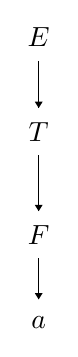
\begin{tikzpicture}[scale=0.1]
	\tikzstyle{every node}+=[inner sep=0pt]
	\draw (31.3,-11.1) node {$E$};
	\draw (31.3,-23.1) node {$T$};
	\draw (31.3,-47.4) node {$a$};
	\draw (31.3,-36.2) node {$F$};
	\draw [black] (31.3,-14.1) -- (31.3,-20.1);
	\fill [black] (31.3,-20.1) -- (31.8,-19.3) -- (30.8,-19.3);
	\draw [black] (31.3,-26.1) -- (31.3,-33.2);
	\fill [black] (31.3,-33.2) -- (31.8,-32.4) -- (30.8,-32.4);
	\draw [black] (31.3,-39.2) -- (31.3,-44.4);
	\fill [black] (31.3,-44.4) -- (31.8,-43.6) -- (30.8,-43.6);
	\end{tikzpicture}
\end{center}

\textbf{Derivation} for $a$: $E \rightarrow T \rightarrow F \rightarrow a$ \\

\textbf{b.} Parse tree for $a + a$: \\
\begin{center}
	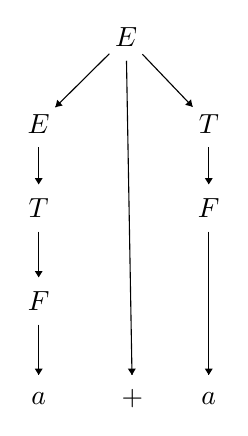
\begin{tikzpicture}[scale=0.1]
	\tikzstyle{every node}+=[inner sep=0pt]
	\draw (42.4,-7.5) node {$E$};
	\draw (31.3,-18.5) node {$E$};
	\draw (31.3,-41) node {$F$};
	\draw (31.3,-29.2) node {$T$};
	\draw (31.3,-53.4) node {$a$};
	\draw (43.2,-53.4) node {$+$};
	\draw (52.9,-53.4) node {$a$};
	\draw (52.9,-18.5) node {$T$};
	\draw (52.9,-29.2) node {$F$};
	\draw [black] (40.27,-9.61) -- (33.43,-16.39);
	\fill [black] (33.43,-16.39) -- (34.35,-16.18) -- (33.65,-15.47);
	\draw [black] (31.3,-21.5) -- (31.3,-26.2);
	\fill [black] (31.3,-26.2) -- (31.8,-25.4) -- (30.8,-25.4);
	\draw [black] (31.3,-32.2) -- (31.3,-38);
	\fill [black] (31.3,-38) -- (31.8,-37.2) -- (30.8,-37.2);
	\draw [black] (31.3,-44) -- (31.3,-50.4);
	\fill [black] (31.3,-50.4) -- (31.8,-49.6) -- (30.8,-49.6);
	\draw [black] (42.45,-10.5) -- (43.15,-50.4);
	\fill [black] (43.15,-50.4) -- (43.63,-49.59) -- (42.63,-49.61);
	\draw [black] (44.47,-9.67) -- (50.83,-16.33);
	\fill [black] (50.83,-16.33) -- (50.64,-15.41) -- (49.91,-16.1);
	\draw [black] (52.9,-21.5) -- (52.9,-26.2);
	\fill [black] (52.9,-26.2) -- (53.4,-25.4) -- (52.4,-25.4);
	\draw [black] (52.9,-32.2) -- (52.9,-50.4);
	\fill [black] (52.9,-50.4) -- (53.4,-49.6) -- (52.4,-49.6);
	\end{tikzpicture}
\end{center}

\textbf{Derivation} for $a + a$: $E \rightarrow E + T \rightarrow T + T 
\rightarrow T + F \rightarrow F + a \rightarrow a + a$ \\

\pagebreak
\textbf{c.} Parse tree for $a + a + a$: \\
\begin{center}
	\begin{tikzpicture}[scale=0.2]
	\tikzstyle{every node}+=[inner sep=0pt]
	\draw (42.4,-7.5) node {$E$};
	\draw (15.4,-22.9) node {$E$};
	\draw (15.4,-42.7) node {$F$};
	\draw (15.4,-32.7) node {$T$};
	\draw (15.4,-52.4) node {$a$};
	\draw (43.3,-52.4) node {$+$};
	\draw (52.9,-52.4) node {$a$};
	\draw (52.9,-18.5) node {$T$};
	\draw (52.9,-32.7) node {$F$};
	\draw (24.2,-11.6) node {$E$};
	\draw (32.3,-22.9) node {$T$};
	\draw (32.3,-52.4) node {$a$};
	\draw (24.2,-52.4) node {$+$};
	\draw [black] (15.4,-25.9) -- (15.4,-29.7);
	\fill [black] (15.4,-29.7) -- (15.9,-28.9) -- (14.9,-28.9);
	\draw [black] (15.4,-35.7) -- (15.4,-39.7);
	\fill [black] (15.4,-39.7) -- (15.9,-38.9) -- (14.9,-38.9);
	\draw [black] (15.4,-45.7) -- (15.4,-49.4);
	\fill [black] (15.4,-49.4) -- (15.9,-48.6) -- (14.9,-48.6);
	\draw [black] (42.46,-10.5) -- (43.24,-49.4);
	\fill [black] (43.24,-49.4) -- (43.72,-48.59) -- (42.72,-48.61);
	\draw [black] (44.47,-9.67) -- (50.83,-16.33);
	\fill [black] (50.83,-16.33) -- (50.64,-15.41) -- (49.91,-16.1);
	\draw [black] (52.9,-21.5) -- (52.9,-29.7);
	\fill [black] (52.9,-29.7) -- (53.4,-28.9) -- (52.4,-28.9);
	\draw [black] (52.9,-35.7) -- (52.9,-49.4);
	\fill [black] (52.9,-49.4) -- (53.4,-48.6) -- (52.4,-48.6);
	\draw [black] (26.504,-9.684) arc (124.87897:80.51176:17.638);
	\fill [black] (26.5,-9.68) -- (27.45,-9.64) -- (26.87,-8.82);
	\draw [black] (22.36,-13.97) -- (17.24,-20.53);
	\fill [black] (17.24,-20.53) -- (18.13,-20.21) -- (17.34,-19.59);
	\draw [black] (25.95,-14.04) -- (30.55,-20.46);
	\fill [black] (30.55,-20.46) -- (30.49,-19.52) -- (29.68,-20.1);
	\draw [black] (24.2,-14.6) -- (24.2,-49.4);
	\fill [black] (24.2,-49.4) -- (24.7,-48.6) -- (23.7,-48.6);
	\draw [black] (32.3,-25.9) -- (32.3,-49.4);
	\fill [black] (32.3,-49.4) -- (32.8,-48.6) -- (31.8,-48.6);
	\end{tikzpicture}
\end{center}

\textbf{Derivation} for $a + a + a$: $E \rightarrow E + T 
\rightarrow T + T + T \rightarrow F + T + F \rightarrow$ \\
$F + F + T \rightarrow F + F + F \rightarrow a + F + F 
\rightarrow a + a + F \rightarrow a + a + a$ \\

\pagebreak
\textbf{d.} Parse tree for $((a))$: \\
\begin{center}
	\begin{forest}
		[E [T [F [(E) [(T) [(F) [((E)) [((T)) [((F)) [a]]]]]]]]]]]
	\end{forest}
\end{center}

\textbf{Derivation} for $((a))$:  $E \rightarrow T \rightarrow F \rightarrow (E) \rightarrow (T) \rightarrow (F) \rightarrow ((E)) $  \\
$ \rightarrow ((T)) \rightarrow ((F)) \rightarrow ((a)) $ \\

%*********************************************************************************
% 2.4 b, c, e, f here

\pagebreak
2.4 \\
Give context-free grammars that generate the following languages. \\
In all parts, the alphabet $\sum$ is $\{0,1\}$. \\

\textbf{b.} \{w| w starts and ends with the same symbol\} \\
$ S \rightarrow 0P0|1P1| \epsilon $ \\
$ P \rightarrow 0P|1P| \epsilon $ \\

\textbf{c.} \{w| the length of w is odd\} \\
$ S \rightarrow 0|1|00S|01S|10S|11S $ \\

\textbf{e.} \{w| w = $w\textsuperscript{R}$, that is, w is a palindrome\} \\
$ S \rightarrow 0|1|0S0|1S1| \epsilon $ \\

\textbf{f.} The empty set \\
$ S \rightarrow \epsilon $ \\

%*********************************************************************************
% 2.5 here

\pagebreak
2.5 Give informal descriptions and state diagrams of pushdown automata for \\
the languages in Exercise 2.4. \\

\textbf{a.} \{w| w contains at least three 1s\}

\textbf{Informal:} In this grammar, there is no need of a stack (as seen in the diagram). In the grammar only the input is read, and the input is only accepted when there is at least three 1's. The only time the machine will accept a string in this case is when at least three 1's are present; otherwise it is rejected.

\textbf{Pushdown Automata:} \\
\begin{center}
	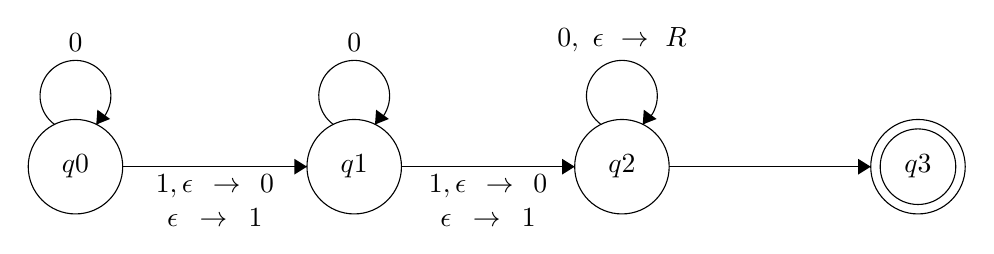
\begin{tikzpicture}[scale=0.2]
	\tikzstyle{every node}+=[inner sep=0pt]
	\draw [black] (12.4,-29.9) circle (3);
	\draw (12.4,-29.9) node {$q0$};
	\draw [black] (30.1,-29.9) circle (3);
	\draw (30.1,-29.9) node {$q1$};
	\draw [black] (47.1,-29.9) circle (3);
	\draw (47.1,-29.9) node {$q2$};
	\draw [black] (65.9,-29.9) circle (3);
	\draw (65.9,-29.9) node {$q3$};
	\draw [black] (65.9,-29.9) circle (2.4);
	\draw [black] (15.4,-29.9) -- (27.1,-29.9);
	\fill [black] (27.1,-29.9) -- (26.3,-29.4) -- (26.3,-30.4);
	\draw (21.25,-30.4) node [below] [text width=2cm,align=center] {$1,\epsilon\mbox{ }\rightarrow\mbox{ }0$\\$\epsilon\mbox{ } \rightarrow\mbox{ }1$};
	\draw [black] (33.1,-29.9) -- (44.1,-29.9);
	\fill [black] (44.1,-29.9) -- (43.3,-29.4) -- (43.3,-30.4);
	\draw (38.6,-30.4) node [below] [text width=2cm,align=center] {$1,\epsilon\mbox{ }\rightarrow\mbox{ }0$\\$\epsilon\mbox{ } \rightarrow\mbox{ } 1$};
	\draw [black] (50.1,-29.9) -- (62.9,-29.9);
	\fill [black] (62.9,-29.9) -- (62.1,-29.4) -- (62.1,-30.4);
	\draw [black] (11.077,-27.22) arc (234:-54:2.25);
	\draw (12.4,-22.65) node [above] {$0$};
	\fill [black] (13.72,-27.22) -- (14.6,-26.87) -- (13.79,-26.28);
	\draw [black] (28.777,-27.22) arc (234:-54:2.25);
	\draw (30.1,-22.65) node [above] {$0$};
	\fill [black] (31.42,-27.22) -- (32.3,-26.87) -- (31.49,-26.28);
	\draw [black] (45.777,-27.22) arc (234:-54:2.25);
	\draw (47.1,-22.65) node [above] {$0,\mbox{ }\epsilon\mbox{ }\rightarrow\mbox{ }R$};
	\fill [black] (48.42,-27.22) -- (49.3,-26.87) -- (48.49,-26.28);
	\end{tikzpicture} \\
\end{center}

\textbf{b.} \{w| w starts and ends with the same symbol\}

\textbf{Informal:} In this grammar, there is an assumption that there is only one symbol in the string
that can be accepted without the use of a stack. If there is more than one symbol in the string,
then all of the symbols are put into the stack in order. We also check to see whether the last
symbol is the one being read. If it is, and this symbol matches with the symbol on the stack,
and if all the input has been checked with no input left, then we accept that state. Otherwise
we reject the input. 

\textbf{Pushdown Automata:} \\
\begin{center}
	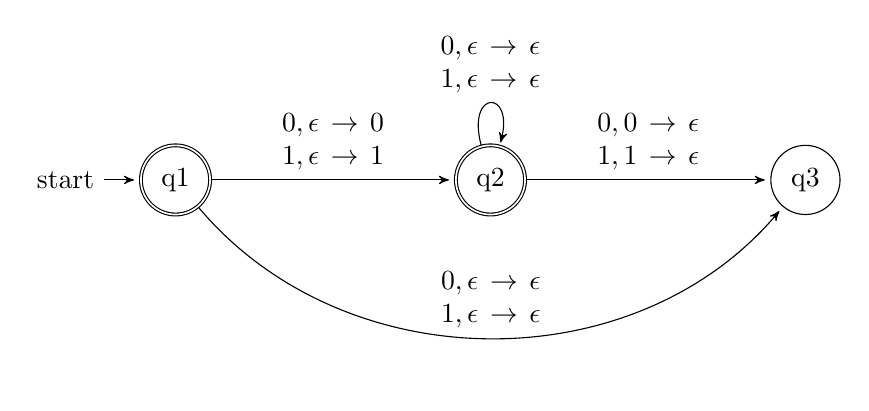
\begin{tikzpicture}[>=stealth',shorten >=2pt, auto, node distance=4cm]
	% Nodes {q1, q2, q3, q4, q5, etc}
	\node [state, initial, accepting] 		(q1) 				 {q1};
	\node [state, accepting] 				(q2)  [right of=q1]  {q2};
	\node [state]   	                    (q3)  [right of=q2]  {q3};

	% Paths
	\path [->] 	(q1) edge 	node	[text width=2cm,align=center]
	{$0, \epsilon \rightarrow 0$ \\ $1, \epsilon \rightarrow 1$}	(q2);

	\path [->] 	(q2) edge 	node	[text width=2cm,align=center]
	{$0, 0 \rightarrow \epsilon$ \\ $1, 1 \rightarrow \epsilon$}	(q3);

	\path [->] 	(q2) edge [loop above] 	node	[text width=2cm,align=center]
	{$0, \epsilon \rightarrow \epsilon$ \\ $1, \epsilon \rightarrow \epsilon$}		(q2);

	\path [->] 	(q1) edge [bend right=50] node [text width=2cm,align=center]
	{$0, \epsilon \rightarrow \epsilon$ \\ $1, \epsilon \rightarrow \epsilon$}	(q3);

	\end{tikzpicture}
\end{center}

\textbf{c.} \{w| the length of w is odd\} 

\textbf{Informal:} In this grammar, there is no need of a stack. 
In this grammar, we only read the input and this input is also 
only accepted when there is an odd length. 

\textbf{Pushdown Automata:} \\
\begin{center}
	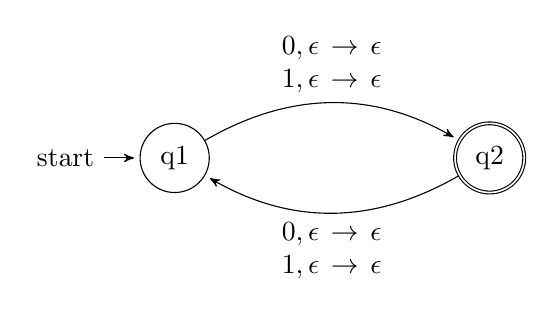
\begin{tikzpicture}[>=stealth',shorten >=2pt, auto, node distance=4cm]
	% Nodes {q1, q2, q3, q4, q5, etc}
	\node [state, initial] 			(q1) 				 {q1};
	\node [state, accepting]        (q2)  [right of=q1]  {q2};

	% Paths
	\path [->] 	(q1) edge [bend left]   node	[text width=2cm,align=center]
	{$0, \epsilon \rightarrow \epsilon$ \\ $1, \epsilon \rightarrow \epsilon$}		(q2);

	\path [->] 	(q2) edge [bend left] 	node	[text width=2cm,align=center]
	{$0, \epsilon \rightarrow \epsilon$ \\ $1, \epsilon \rightarrow \epsilon$}		(q1);

	\end{tikzpicture}
\end{center}

\textbf{d.} \{w| the length of w is odd and its middle symbol is a 0\}

\textbf{Informal:} In this grammar, the input is read by the pushdown automata and each symbol is
placed onto the stack. At each point, the pushdown automata guesses if the input in the middle
or if the next symbol read is in the middle of the string. If the next symbol read is the middle
of the string then it does not get read onto the stack. After this, we pop symbols off the stack
if they match the input symbols that were read. If the symbols that are popped match the symbols
that were pushed earlier, and the stack is empty as the input is finished, we accept the state.
Otherwise we reject the state.

\textbf{Pushdown Automata:} \\
\begin{center}
	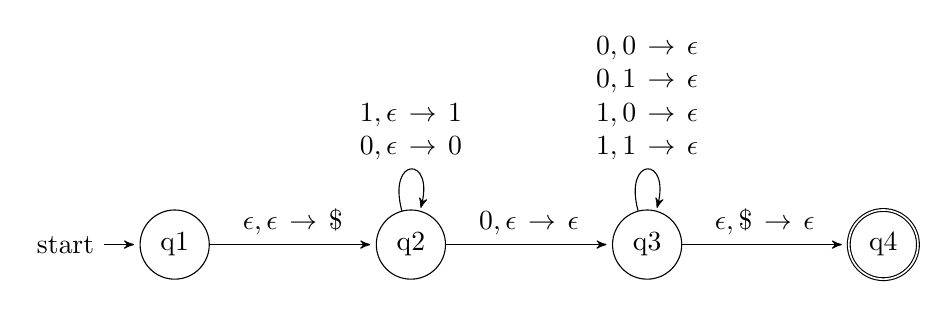
\begin{tikzpicture}[>=stealth',shorten >=2pt, auto, node distance=3cm]
	% Nodes {q1, q2, q3, q4, q5, etc}
	\node [state, initial] 		(q1) 				 {q1};
	\node [state] 				(q2)  [right of=q1]  {q2};
	\node [state]    			(q3)  [right of=q2]  {q3};
	\node [state, accepting]	(q4)  [right of=q3]  {q4};

	% Paths
	\path [->] 	(q1) edge 				node	[text width=2cm,align=center]
	{$\epsilon, \epsilon \rightarrow \$$}	(q2);

	\path [->] 	(q2) edge 				node	[text width=2cm,align=center]
	{$0, \epsilon \rightarrow \epsilon$}	(q3);

	\path [->] 	(q2) edge [loop above] 	node	[text width=2cm,align=center]
	{$1, \epsilon \rightarrow 1$ \\ $0, \epsilon \rightarrow 0$}		(q2);

	\path [->] 	(q3) edge 				node	[text width=2cm,align=center]
	{$\epsilon, \$ \rightarrow \epsilon$}		(q4);

	\path [->] 	(q3) edge [loop above] 	node	[text width=2cm,align=center]
	{$0, 0 \rightarrow \epsilon$ \\ $0, 1 \rightarrow \epsilon$ \\ $1, 0 \rightarrow \epsilon$ \\ $1, 1 \rightarrow \epsilon$}	(q3);

	\end{tikzpicture} \\
\end{center}

\pagebreak
\textbf{e.} \{w| w = $w\textsuperscript{R}$, that is, w is a palindrome\}

\textbf{Informal:} In this grammar, the input is read by the pushdown automata and each symbol is
placed onto the stack. At each point, the pushdown automata guesses if the input in the middle
or if the next symbol read is in the middle of the string. If the next symbol read is the middle
of the string then it does not get read onto the stack. After this, we pop symbols off the stack
if they match the input symbols that were read. If the symbols that are popped match the symbols
that were pushed earlier, and the stack is empty as the input is finished, we accept the state.
Otherwise we reject the state.

\textbf{Pushdown Automata:} \\
\begin{center}
	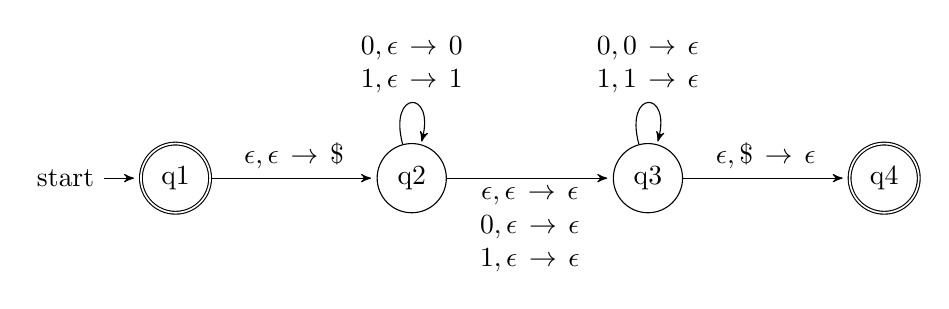
\begin{tikzpicture}[>=stealth',shorten >=2pt, auto, node distance=3cm]
	% Nodes {q1, q2, q3, q4, q5, etc}
	\node [state, initial, accepting] 		(q1) 				 {q1};
	\node [state] 				(q2)  [right of=q1]  {q2};
	\node [state]    			(q3)  [right of=q2]  {q3};
	\node [state, accepting]	(q4)  [right of=q3]  {q4};

	% Paths
	\path [->] 	(q1) edge 				node	[text width=2cm,align=center]
	{$\epsilon, \epsilon \rightarrow \$$}	(q2);

	\path [->] 	(q2) edge 	[below]	node	[text width=2cm,align=center]
	{$\epsilon, \epsilon \rightarrow \epsilon$ \\ $0, \epsilon \rightarrow \epsilon$ \\ $1, \epsilon \rightarrow \epsilon$}	(q3);

	\path [->] 	(q2) edge [loop above] 	node	[text width=2cm,align=center]
	{$0, \epsilon \rightarrow 0$ \\ $1, \epsilon \rightarrow 1$}		(q2);

	\path [->] 	(q3) edge 				node	[text width=2cm,align=center]
	{$\epsilon, \$ \rightarrow \epsilon$}		(q4);

	\path [->] 	(q3) edge [loop above] 	node	[text width=2cm,align=center]
	{$0, 0 \rightarrow \epsilon$ \\ $1, 1 \rightarrow \epsilon$}	(q3);

	\end{tikzpicture} \\
\end{center}

\textbf{f.} The empty set

\textbf{Informal:} In this grammar, the language only accepts an empty set so it implies that
it does not terminate any derivation. And if none of the derivations are terminated,
that means that no string is accepted by the CFG, including the empty string.

\textbf{Pushdown Automata:} \\
\begin{center}
	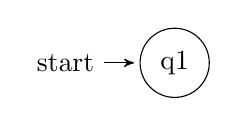
\begin{tikzpicture}[>=stealth',shorten >=2pt, auto, node distance=2cm]
	% Nodes {q1, q2, q3, q4, q5, etc}
	\node [state, initial] 		(q1) 				{q1};

	\end{tikzpicture}
\end{center}

%*********************************************************************************
% 2.6 here

\pagebreak
2.6 \\

\textbf{b.} The complement of the language $\{a^nb^n \; | \; n >= 0\}$
The language is: \\
$S \rightarrow S_1 \quad | \quad S_2$ \\
$S_1 \rightarrow a S_1 b \quad | \quad T \quad | \quad U$   \\
$S_2 \rightarrow RbaR$ \\
$T \rightarrow aT \quad | \quad a$ \\
$U \rightarrow Ub \quad | \quad a$ \\
$R \rightarrow RR \quad | \quad a \quad | \quad b \quad | \quad \epsilon$ \\

\textbf{d.} $\{x_1\#x_2\# \; ... \; \#x_k \; | \; k \geq 1, each \; x_i \epsilon \{a, b\}^*, and \; for \; some \; i \; and \; j, \; x_i = x^R_j\}$
The language is: \\
$R \rightarrow S \quad | \quad J\#S\#J \quad | \quad J\#S \quad | \quad S\#J$ \\
$S \rightarrow aSa \quad | \quad bSb \quad | \quad \# \quad | \quad \#J\#$ \\
$J \rightarrow aJ \quad | \quad bJ \quad | \quad \#J \quad | \quad \epsilon$ \\

%*********************************************************************************
% 2.9 here
\pagebreak

2.9 $A = \{ a^i b^j c^k \; \; | \; i = j \; or \; j = k, \; where \; i, j, k \geq 0\}$ \\
The context free grammar that generates the language is: \\

First, split the languages into two parts: \\
$A_1 = \{ a^i b^j c^k \; \; | \; \; i,j,k \geq 0, \; i = j \}$ \\
$A_2 = \{ a^i b^j c^k \; \; | \; \; i,j,k \geq 0, \; j= k \}$ \\

Now we can define the grammar for the language A: \\
$S \rightarrow S_1 \; | \; S_2$ \\

In $A_1$, the values of i and j are equal. So, there must be an equal number
of A's and B's in this language. \\

CGF for language $A_1$ is: \\
$S_1 \rightarrow S_1 c \; | \; E \; | \; \epsilon $ \\
$E \rightarrow aEb \; | \; \epsilon  $ \\

In $A_2$, j and k are equal, so there are an equal number of B'c and C's. \\

CGF for language $A_2$ is: \\
$S_2 \rightarrow a S_2 \; | \; F \; | \; \epsilon $ \\
$F \rightarrow bFc \; | \; \epsilon  $ \\

Since we can use either $A_1$ or $A_2$ to generate the string, either $S_1$ or
$S_2$ can be used. Thus, the context free grammar for the language A is ambiguous. \\

%*********************************************************************************
% 2.10 here
\pagebreak

2.10 Give an informal description of a pushdown automaton that recognizes the language A in Exercise 2.9. \\

At the beginning, we break into two branches. In the first branch, for each a that is read,
we push an a onto the stack. Then, we guess when the first b is read, and begin popping
symbols from the stack for every b that we read. When the stack is empty, the only input
that is remaining should be C, and then we read the input without adjusting the stack.
If we read the symbols in the proper order, that is a followed by b followed by c,
and the stack is empty by the time the B's are done reading, then we accept the state.
Otherwise, we reject the state. \\

In the second branch, for a that we read, we do not adjust the stack. We then guess
when the first b is read and we begin pushing symbols onto the stack for every b that
we read. We then guess when the first c is read - and we begin popping symbols from the
stack for every c that is read. If the stack becomes empty right when the input string
is finished, and the symbols were read in the right order, we accept. Otherwise, we
reject the state. \\

%*********************************************************************************
% 2.11 here
\pagebreak

2.11 Convert the CFG $G_4$ given in Exercise 2.1 to an equivalent PDA, 
using the procedure given in Theorem 2.20. \\

Given CFG: \\
$E \rightarrow E + T \; | \; T $ \\
$E \rightarrow T \times F \; | \; F $ \\
$F \rightarrow (E) \; | \; a $ \\

\textbf{PDA for $G_4$:} \\

\begin{center}
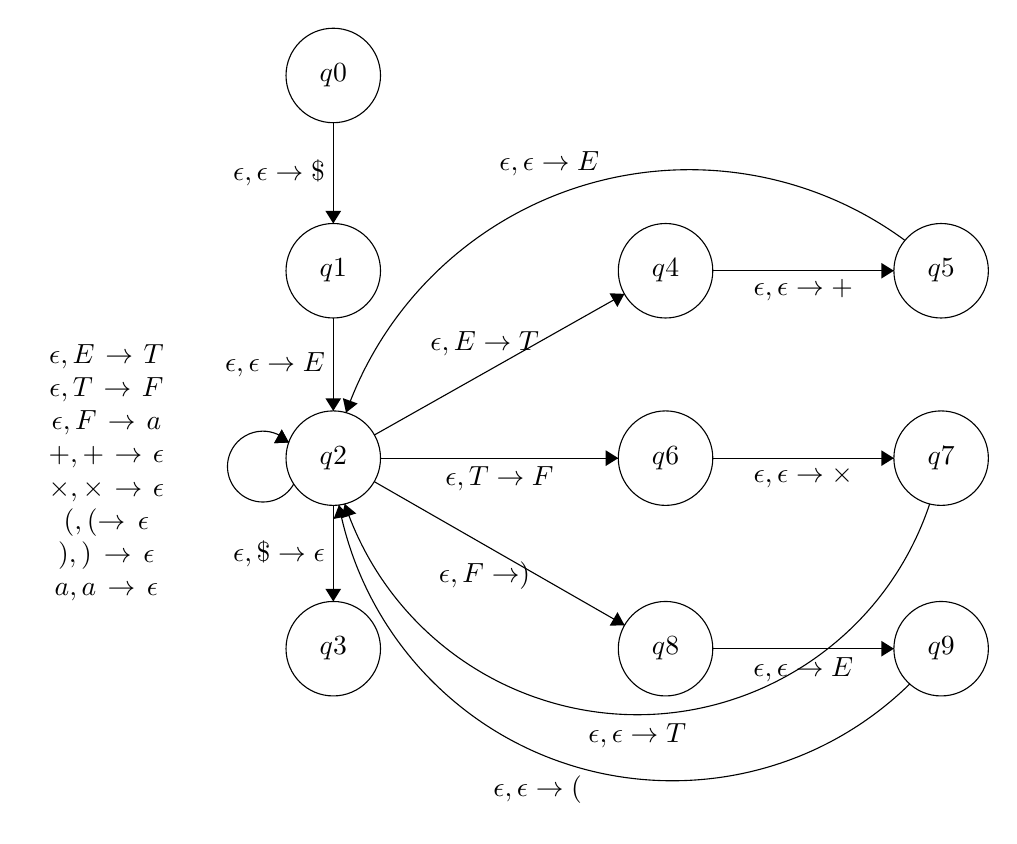
\begin{tikzpicture}[scale=0.2]
\tikzstyle{every node}+=[inner sep=0pt]
\draw [black] (17.1,-5.2) circle (3);
\draw (17.1,-5.2) node {$q0$};
\draw [black] (17.1,-17.6) circle (3);
\draw (17.1,-17.6) node {$q1$};
\draw [black] (17.1,-29.5) circle (3);
\draw (17.1,-29.5) node {$q2$};
\draw [black] (17.1,-41.6) circle (3);
\draw (17.1,-41.6) node {$q3$};
\draw [black] (38.2,-17.6) circle (3);
\draw (38.2,-17.6) node {$q4$};
\draw [black] (55.7,-17.6) circle (3);
\draw (55.7,-17.6) node {$q5$};
\draw [black] (38.2,-29.5) circle (3);
\draw (38.2,-29.5) node {$q6$};
\draw [black] (55.7,-29.5) circle (3);
\draw (55.7,-29.5) node {$q7$};
\draw [black] (38.2,-41.6) circle (3);
\draw (38.2,-41.6) node {$q8$};
\draw [black] (55.7,-41.6) circle (3);
\draw (55.7,-41.6) node {$q9$};
\draw [black] (17.1,-8.2) -- (17.1,-14.6);
\fill [black] (17.1,-14.6) -- (17.6,-13.8) -- (16.6,-13.8);

% Right nodes here
\draw (16.6,-11.4) node [left] {$\epsilon, \epsilon \rightarrow \$$};
\draw [black] (17.1,-20.6) -- (17.1,-26.5);
\fill [black] (17.1,-26.5) -- (17.6,-25.7) -- (16.6,-25.7);
\draw (16.6,-23.55) node [left] {$\epsilon, \epsilon \rightarrow E$};
\draw [black] (17.1,-32.5) -- (17.1,-38.6);
\fill [black] (17.1,-38.6) -- (17.6,-37.8) -- (16.6,-37.8);
\draw (16.6,-35.55) node [left] {$\epsilon, \$ \rightarrow \epsilon$};

% q4 + q5 nodes
\draw [black] (19.71,-28.03) -- (35.59,-19.07);
\fill [black] (35.59,-19.07) -- (34.64,-19.03) -- (35.14,-19.9);
\draw (26.71,-23.05) node [above] {$\epsilon, E \rightarrow T$};
\draw [black] (41.2,-17.6) -- (52.7,-17.6);
\fill [black] (52.7,-17.6) -- (51.9,-17.1) -- (51.9,-18.1);
\draw (46.95,-18.1) node [below] {$\epsilon, \epsilon \rightarrow +$};

%\draw (65.3,-18.1) node [below] {$\epsilon, \epsilon \rightarrow E$};

% q6 + q7 nodes
\draw [black] (20.1,-29.5) -- (35.2,-29.5);
\fill [black] (35.2,-29.5) -- (34.4,-29) -- (34.4,-30);
\draw (27.65,-30) node [below] {$\epsilon, T \rightarrow F$};
\draw [black] (41.2,-29.5) -- (52.7,-29.5);
\fill [black] (52.7,-29.5) -- (51.9,-29) -- (51.9,-30);
\draw (46.95,-30) node [below] {$\epsilon, \epsilon \rightarrow \times$};

%\draw (65.3,-30) node [below] {$\epsilon, \epsilon \rightarrow T$};

% q8 + q9 nodes
\draw [black] (19.7,-30.99) -- (35.6,-40.11);
\fill [black] (35.6,-40.11) -- (35.15,-39.28) -- (34.65,-40.14);
\draw (26.71,-36.05) node [below] {$\epsilon, F \rightarrow )$};
\draw [black] (41.2,-41.6) -- (52.7,-41.6);
\fill [black] (52.7,-41.6) -- (51.9,-41.1) -- (51.9,-42.1);
\draw (46.95,-42.1) node [below] {$\epsilon, \epsilon \rightarrow E$};

%\draw (65.3,-42.1) node [below] {$\epsilon, \epsilon \rightarrow ($};

% Bends
% q5 bend
\fill [black] (14.28,-28.51) -- (13.83,-27.68) -- (13.34,-28.55);
\draw [black] (17.911,-26.614) arc (160.58185:53.68618:23.118);
\fill [black] (17.91,-26.61) -- (18.65,-26.03) -- (17.71,-25.69);
\draw (30.82,-11.6) node [above] {$\epsilon, \epsilon \rightarrow E$};

% q7 bend
\draw [black] (54.972,-32.407) arc (-18.45344:-161.54656:19.578);
\fill [black] (17.83,-32.41) -- (17.61,-33.32) -- (18.56,-33.01);
\draw (36.4,-46.29) node [below] {$\epsilon, \epsilon \rightarrow T$};

% q9 bend
\draw [black] (53.708,-43.84) arc (-45.63394:-169.1755:21.559);
\fill [black] (17.46,-32.48) -- (17.12,-33.36) -- (18.1,-33.17);
\draw (30.08,-49.61) node [below] {$\epsilon, \epsilon \rightarrow ($};

% Loop
\draw [black] (14.597,-31.132) arc (-29.16862:-317.16862:2.25);
\draw (7.73,-30.43) node [left] [text width=2cm,align=center]
{$\epsilon, E \rightarrow T$ \\ $\epsilon, T \rightarrow F$ \\
 $\epsilon, F \rightarrow a$ \\ $+,+ \rightarrow \epsilon$ \\
 $\times, \times \rightarrow \epsilon$ \\ $(, ( \rightarrow \epsilon$ \\
 $), ) \rightarrow \epsilon$ \\ $a,a \rightarrow \epsilon$ };

%\draw (9.73,-30.43) node [left] [text width=2cm,align=center] {$\epsilon,E\mbox{ }\rightarrow\mbox{ }0$\\$\epsilon\mbox{ } \rightarrow\mbox{ }1$};
\fill [black] (14.28,-28.51) -- (13.83,-27.68) -- (13.34,-28.55);
\end{tikzpicture}
\end{center}

%*********************************************************************************
% 2.12 here
\pagebreak

2.12 Convert the CFG G given in Exercise 2.1 to an equivalent PDA, using the procedure given in Theorem 2.20. \\

\textbf{CFG} $G$ given in 2.3: \\
$R \rightarrow XRX \; | S\; $ \\
$S \rightarrow aTb \; | \; bTa $ \\
$T \rightarrow XTX \; | \; X \; | \; \epsilon $ \\
$X \rightarrow a \; | \; b $ \\

\textbf{PDA for $G$:} \\

\begin{center}
	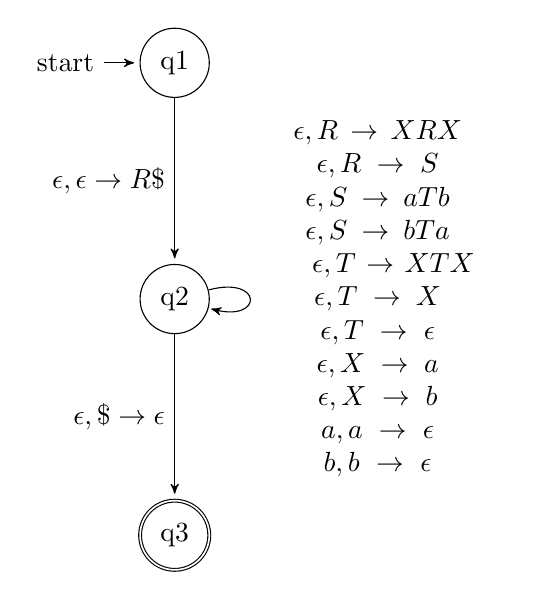
\begin{tikzpicture}[>=stealth',shorten >=2pt, auto, node distance=3cm]
	% Nodes {q1, q2, q3, q4, q5, etc}
	\node [state, initial] 		(q1) 				 {q1};
	\node [state] 				(q2)  [below of=q1]  {q2};
	\node [state, accepting]	(q3)  [below of=q2]  {q3};

	% Top path
	\path [->] 	(q1) edge 	[left]			node
	{$\epsilon, \epsilon \rightarrow R\$$}		(q2);

	% Bottom path
	\path [->] 	(q2) edge 	[left]			node
	{$\epsilon,\$ \rightarrow \epsilon$}		(q3);

	% Super long loop
	\path [->] 	(q2) edge [loop right] 	node	[text width=3cm,align=center]
	{$\epsilon, R \rightarrow XRX$ \\ $\epsilon, R \rightarrow S$ \\
	 $\epsilon, S \rightarrow aTb$ \\ $\epsilon, S \rightarrow bTa$ \\
	 $ \; \; \; \epsilon, T \rightarrow XTX$ \\ $\epsilon, T \rightarrow X$ \\
	 $\epsilon, T \rightarrow \epsilon$ \\ $\epsilon, X \rightarrow a$ \\
	 $\epsilon, X \rightarrow b$ \\ $a, a \rightarrow \epsilon$ \\
	 $b, b \rightarrow \epsilon$}		(q2);

	\end{tikzpicture} \\
\end{center}

%*********************************************************************************
% 2.13 here
\pagebreak
2.13 Let $G = (V, \sum, R, S)$ be the following grammar, \\
$V = \{S, T, U\}; Σ = \{0, \#\};$ \\

and $R$ is the set of rules: \\
$S \rightarrow TT \; | \; U$ \\
$T \rightarrow 0T \; | \; T 0 \; | \; \#$ \\
$U \rightarrow 0U 00 \; | \; \#$ \\

\underline{\textbf{a)}} Describe L(G) in English. \\

$L(G)$ is the set of all strings that contain a string of 0's, and all \#'s of the
following forms: \\

\textbf{1.} Strings which contain exactly two \#'s. \\
\textbf{2.} Strings that contain two \#'s in the middle of the string, and any number of 0's
on either sides of the string. \\
\textbf{3.} Strings that contain exactly one \#, and the number of 0's to the left of the \#
are half the number of 0's that are to the right. \\

\underline{\textbf{b)}} Prove that L(G) is not regular. \\

To prove that $L(G)$ is not regular, we will need to do a proof by contradiction that
states that $L(G)$ is regular. Let us define A: \\

$A = L(G) \bigcup 0^* \# 0^*$

We assume that $L(G)$ is regular, so A is regular too. Since A is regular, we can use
pumping lemma to let $p$ be the pumping length fo the regular language. \\

We can now consider the string $w = 0^p \# 0^{2p} $ \\
It seems clear that the length of $w \; \in \; A$ is greater than $p$. This means
that $|w| > p$. By pumping lemma, we now have $w = xyz$ such that:

$|xy| \le p, y \neq \epsilon $ and $xy^iz \in L(G)$ for all $i \geq 0$ \\

\pagebreak
Since A is a regular language, we can now consider all the possible ways of cutting
the string $w$: \\

\textbf{1.} If $x$ contains the character \#, then $y$ will be on the right side of the \#.
As we pump $y$ down, it increases the number of 0's on the left so that the number of
0's on the left of the \# is not equal to half of the number of 0's to the right of the \#.

\textbf{2.} If $y$ contains a \#, then as we pump $y$ down, it increases the number of \#'s in the string.

\textbf{3.} If $z$ contains a \#, then $y$ should be on the left side of the \#. As we pump $y$ down in this
case, it decreases the number of 0's to the right, such that the number of 0's to the left of the \#
are not equal to half the number of 0's to the right of the \#. \\

The string that results from the above cases does not belong to $A$. As a result, we can say that
$A$ does not satisfy the pumping lemma. Basically, $A$ is not a regular language. This is a
contradiction to the statement that we assumed at the beginning of this proof:
$L(G)$ is a regular language. Thus, \underline{\textbf{$L(G)$ is not a regular language.}}

%*********************************************************************************
% 2.14 here
\pagebreak
2.14 Convert the following CFG into an equivalent CFG in Chomsky normal form,
using the procedure given in Theorem 2.9. \\

$A \rightarrow BAB \; | \; B \; | \; \epsilon $ \\
$B \rightarrow 00 \; | \; \epsilon $ \\

Let's use the \textbf{Chomsky Normal Form} to solve this problem. For a CFG to be in
the \textbf{Chomsky Normal Form}, it must follow the following rules:

$A \rightarrow BC$ \\
$A \rightarrow a$  \\

Where: $a$ is any terminal, $A$, $B$, and $C$ are any variables, except that B and C may not be the starting variable.
We also have the rule $S \rightarrow \epsilon$, which is where $S$ is the starting variable. \\

With this in mind, we can now convert the given CFG to an equivalent CFG in CNF form.
We will have the above rules, as well as another starting variable and rule. The grammar
would therefore start out as: \\
$S_0 \rightarrow A$ \\
$A \rightarrow BAB \; | \; B \; | \; \epsilon $ \\
$B \rightarrow 00 \; | \; \epsilon $ \\

We now need to start removing all rules that contain $\epsilon$. We will remove the rule
$A \rightarrow \epsilon$ and the rule $B \rightarrow \epsilon$. This gives us the following
grammar:

$S_0 \rightarrow A \; | \; \epsilon$ \\
$A \rightarrow BAB \; | \; BA \; | \; AB \; | \; A \; | \; B \; | \; BB $ \\
$B \rightarrow 00 $ \\

$S_0 \rightarrow A \; | \; \epsilon$ is acceptable since $S_0$ is the starting variable,
and this is allowed in \textbf{Chomsky Normal Form}. We can now rule the unit rules: \\

Removing $A \rightarrow A$ will give us: \\
$S_0 \rightarrow A \; | \; \epsilon$ \\
$A \rightarrow BAB \; | \; BA \; | \; AB \; | \; B \; | \; BB $ \\
$B \rightarrow 00 $ \\

\pagebreak

Removing $S \rightarrow B$ will give us: \\
$S_0 \rightarrow A \; | \; \epsilon$ \\
$A \rightarrow BAB \; | \; BA \; | \; AB \; | \; 00 \; | \; BB $ \\
$B \rightarrow 00 $ \\

Removing $S_0 \rightarrow S$ will give us: \\
$S_0 \rightarrow BAB \; | \; BA \; | \; AB \; | \; 00 \; | \; BB \; | \; \epsilon$ \\
$A \rightarrow BAB \; | \; BA \; | \; AB \; | \; 00 \; | \; BB $ \\
$B \rightarrow 00 $ \\

We can also replace all of the terminal 0's with a new variable, $U$, as such:
$S_0 \rightarrow BAB \; | \; BA \; | \; AB \; | \; 00 \; | \; BB \; | \; \epsilon$ \\
$A \rightarrow BAB \; | \; BA \; | \; AB \; | \; 00 \; | \; BB $ \\
$B \rightarrow UU $ \\
$U \rightarrow 0$ \\

We can now shorten the right hand side of the rules by using only 2 variables each.
To shortern these rules we will replace $S_0 \rightarrow BAB$ with two new rules: \\
$S_0 \rightarrow BA_1$ and \\
$A_1 \rightarrow AB$ \\

We can also replace the rule $A \rightarrow BAB$ with two new rules: \\
$A \rightarrow BA_2$ and \\
$A_2 \rightarrow AB$ \\

After we replace these rules, the final CFG in \textbf{Chomsky Normal Form} is: \\
$G = (V, \sum, R, S_0$ \\
set of rules $V = \{S_0, S, B, U, A_1, A_2 \}$ \\
starting variable: $S_0$ \\
The set of terminals: $\sum = \{ 0 \}$ \\
Rules $R$ given by: \\
$S_0 \rightarrow BA_1 \; | \; BA \; | \; SB \; | \; UU \; | \; BB \; | \; \epsilon$ \\
$A \rightarrow BA_2 \; | \; BA \; | \; SB \; | \; UU \; | \; BB $ \\
$B \rightarrow UU $ \\
$U \rightarrow 0$ \\
$A_1 \rightarrow AB$ \\
$A_2 \rightarrow AB$ \\

%*********************************************************************************
% 2.26 here
\pagebreak

2.26 \\
Show that if $G$ is a CFG in \textbf{Chomsky Normal Form} form, then for any string $w \; \in \; L(G)$
of length $n \geq 1$, exactly $2n - 1$ steps are required for any derivation of $w$. \\

We can prove that $G$ is in CNF form by using the induction method on the string $w$ of length $n$. \\

Let's do this as follows: \\
$N = 1$, a string "a" is of length 1 in CNF form, so derivation that is valid for this is
$S \rightarrow a$ where $a \in \sum$ and $S$ is the starting symbol. \\

The number of steps required can be found by doing: \\
$2n - 1 = 2(1) - 1$ \\
$ \quad = 2 - 1 $ \\
$       = 1 $ \\
Thus it is true that for $n = 1$ that $2n - 1$ steps are required to derive a string a. \\

Now we can find the steps required for the case $n = k$. This would be a string of length
$k \geq n$ in CNF form, so a valid derivation for this should take $2k - 1$ steps. \\

The number of steps required can be found by doing: \\
$2n - 1 = 2(k) - 1$ \\
$       = 2k - 1 $ \\

We will assume a string length of at most $k \geq n$ terminal symbols, and that it has a string
length of $n = k + 1$ in CNF form. \\

Since we know that $n > 1$, we can consider a language that follows CNF:
$S \rightarrow BC$ \\
$B \rightarrow *x$ \\
$C \rightarrow *y$ \\

Where the derivation starts with the given symbol $S$. The length of the string with
this starting symbol $S$ is $|w| = xy$ where $|x| > 0$ and $|y| > 0$. \\

We can use the inductive hypothesis now: \\

$1 + (2 |x| - 1) + (2 |y| - 1) = 2|x| + 2|y| + 1 - 1 - 1 = 2 (|x| + |y|) - 1 $ \\

Which shows that $n = |x| + |y|$. \\

We've found that $B \rightarrow *x$ has a length of $|x|$ and that $C \rightarrow *y$
has a length $|y|$. Thus, it is proven that it requires $2n - 1$ steps to get the
derivation of the string $w \in L(G)$ in \textbf{CNF} form.

%*********************************************************************************
% 2.30 here
\pagebreak
2.30 Use the pumping lemma to show that the following languages are not context free. \\

\textbf{a.} Given language is: $ \{0^n 1^n 0^n 1^n \; | \; n \geq 0 \} $ \\

Let $A = \{0^n 1^n 0^n 1^n \; | \; n \geq 0 \} $ \\
$p$ will be there pumping length of $A$ given by pumping lemma. \\

We can now prove that $A$ is not a \textbf{Context-Free Language (CFL)}.
In order to prove this, we will need to show that a string $s = 1^p 0^p 1^p 0^p$
cannot be pumped. We will consider $s$ in the form of $s = uvxyz$. \\

1. If both $v$ and $y$ contain at most one alphabet symbol type, the string
will be in the form of $u v^2 x y^2 z$, which is a string of $0's$ and $1's$
of unequal length. In this case, the string $s$ cannot be a member of $A$. \\

2. If either $v$ or $y$ contain more than one alphabet symbol type, the string
will end up in the form of $u v^2 x y^2 z$ which does not contain the
symbols in the required order. In this case, the string $s$ cannot be a
member of $A$. \\

Since we cannot pump the string $s$ without violating the conditions of
pumping lemma, $A$ is not a \textbf{CFL}. \\


\textbf{b.} $\{0^n \# 0^{2n} \# 0^{3n} \; | \; n \geq 0 \} $ \\

Let $B = \{0^n \# 0^{2n} \# 0^{3n} \; | \; n \geq 0 \} $ \\
$p$ will be there pumping length of $B$ given by pumping lemma. \\

We can now prove that $B$ is not a \textbf{Context-Free Language (CFL)}.
In order to show this, we will consider the string $s = 0^p \# 0^{2p} \# 0^{3p}$,
and we will show that string $s$ cannot be pumped by pumping lemma. We will
consider $s$ in the form of $s = uvxyz$. \\

1. Neither $v$ nor $y$ can contain the symbol $\#$, otherwise $x v^2 w y^2 z$
will contain more than two "\#" symbols. If this string is divided into
three segments of $\#$s, then at least one of the segments $0^p$,
$0^{2p}$, and $0^{3p}$ cannot be contained within either $v$ or $y$. \\

2. Because the ratio of length between the segments is not maintained in
a $1:2:3$ ratio, $x v^2 w y^2 z$ cannot be contained within $B$.
Which means that string $s$ cannot be a member of $B$. \\

Since we cannot pump the string $s$ without violating the conditions of
pumping lemma, $B$ is not a \textbf{CFL}. \\


\textbf{c.} $\{ w \# t \; | \; w$ is a substring of $t$, where $w$, $t \in \{a, b\}^* \} $ \\

Let $C = \{ w \# t \; | \; w$ is a substring of $t$, where $w$, $t \in \{a, b\}^* \}$ \\
$p$ will be there pumping length of $C$ given by pumping lemma. \\

We can now prove that $C$ is not a \textbf{Context-Free Language (CFL)}.
In order to show this, we will consider the string $s = a^p b^p \# a^p b^p $,
and we will show that string $s$ cannot be pumped by pumping lemma. We will
consider $s$ in the form of $s = uvxyz$. \\

1. Neither $v$ nor $y$ can contain a symbol $\#$, otherwise $u v^0 x y^0 z$
will not contain a $\#$. In this case, string $s$ cannot be a member of $C$. \\

2. If both $v$ and $y$ are not empty, and they both occur on the left side of the
$\#$, then the string $u v^2 x y^2 z$ is no longer on the left side of the
$\#$ symbol. In this case, string $s$ cannot be a member of $C$. \\

3. We can also consider when both $v$ and $y$ are not empty, and they both occur
on the right side of the $\#$ symbol. In this case, the string $u v^0 x y^0 z$
is no longer on the right side of the $\#$ symbol. In this case, string $s$
cannot be a member of $C$. \\

4. If just one of either $v$ and $y$ is not empty, then we can assume that they
both occurred on the same side of the $\#$ symbol. In this case, string $s$
cannot be a member of $C$. \\

5. The final case is that if both $v$ and $y$ are not empty and they both
include the $\#$ symbol. Then in this case, by the third pumping lemma
condition of $|vxy| \; \le \; p$, we will end up with $v$ consisting of
$b's$ and $y$ will consist of $a's$. This means that $u v^2 x y^2 z$ contains
more $b's$ on the left side of the $\#$ symbol. In this case, string $s$
cannot be a member of $C$. \\

Since we cannot pump the string $s$ without violating the conditions of
pumping lemma, $C$ is not a \textbf{CFL}. \\


\textbf{d.} $\{t_1 \# t_2 \# ... \# t_k \; | \; k \geq 2$, each $t_i \in \{a, b\}^*$, and $t_i = t_j$ for some $i \ne j \} $ \\

Let $D = \{t_1 \# t_2 \# ... \# t_k \; | \; k \geq 2$, each $t_i \in \{a, b\}^*$, and $t_i = t_j$ for some $i \ne j \} $ \\
$p$ will be there pumping length of $D$ given by pumping lemma. \\

We can now prove that $D$ is not a \textbf{Context-Free Language (CFL)}.
In order to show this, we will consider the string $s = a^p b^p \# a^p b^p $,
and we will show that string $s$ cannot be pumped by pumping lemma. We will
consider $s$ in the form of $s = uvxyz$. \\

1. Neither $v$ nor $y$ can contain a symbol $\#$, otherwise $u v^0 x y^0 z$
will not contain a $\#$. In this case, string $s$ cannot be a member of $C$. \\

2. If just either $v$ or $y$ is not empty, than we can assume that they both occured
on the same side of the $\#$ symbol. In this case, string $s$ cannot be a member of $C$. \\

3. If both $v$ and $y$ are not empty, and they both occur on the left hand side
of the $\#$ symbol, then the string $u v^2 x y^2 z$ is not on the left hand
side of the $\#$. In this case, string $s$ cannot be a member of $C$. \\

4. If both $v$ and $y$ are not empty, and they both occur on the right hand side
of the $\#$ symbol, then the string $u v^0 x y^0 z$ is no longer on the
right hand side of the $\#$. In this case, string $s$ cannot be a member of $C$. \\

5. In the final case, if both $v$ and $y$ are not empty and they both include
the $\#$ symbol, then by the third pumping lemma condition $|vxy| \; \le \; p$,
we have $v$ that consists of $b's$ and $y$ that consists of $a's$. This will
lead to $u v^2 x y^2 z$ containing more $b's$ on the left hand side of the $\#$.
In this case, string $s$ cannot be a member of $C$. \\

Since we cannot pump the string $s$ without violating the conditions of
pumping lemma, $D$ is not a \textbf{CFL}. \\

%*********************************************************************************
% 2.31 here
\pagebreak
2.31 Let B be the language of all palindromes over $\{0, 1\}$ containing equal numbers of
$0s$ and $1s$. Show that $B$ is not context free. \\

To solve this problem, we will assume that $B$ is a \textbf{Context-Free Language (CFL)},
and prove that it is not by contradiction. \\

$p$ will be there pumping length of $B$ given by pumping lemma. \\
We will consider a string $s = 0^p 1^p 1^p 0^p$ \\

We will assume that string $s$ is a member of $B$, and that it has
a length of $p$. We can show that anyway you divide the string into
a form of $uvxyz$, one of the conditions of pumping lemma is violated.
Pumping lemma is where $|xyz| \le p$, and we can only place $xyz$ into
the following ways: \\

\textbf{1.} $vxy$ fails completely in the first $0^p$.

If we pump $v$ and $y$, then the string that is created is no
longer a valid palindrome, and the number of $0s$ will be greater
than the number of $1s$. This is a contradiction.

\textbf{2.} $vxy$ fails between $0^p$ and $1^p$.

If $v$ only contains $0s$ while $y$ only contains $1s$, then
if we pump string $s$, the new string that is created is no
longer a palin drome. This is a contradiction.

\textbf{3.} $vxy$ fails completely in the first $1^p$.

This case is similar to \textbf{1}, after we pump string $s$,
the number of $1s$ will be greater than the number of $0s$,
which is a contradiction.

\textbf{4.} $vxy$ falls between $1^p$ and $1^p$

After pumping the string $s$, the number of $1s$ will be greater
than the number of $0s$, which is a contradiction.

\textbf{5.} $vxy$ falls completely within the second $1^p$

This is the same case as \textbf{3}.

\textbf{6.} $vxy$ falls between $1^p$ and $0^p$

This is similar to case \textbf{2}, $v$ will only contain
$1s$ while $y$ will only contain $0s$. If we pump the string
$s$ then the new string will no longer be a palindrome.
This is a contradiction.

\textbf{7.} $vxy$ falls completely within the second $0^p$

This is the same case as \textbf{1}. \\

As shown above, $B$ is not a \textbf{CFL}.

%*********************************************************************************
% 2.32 here
\pagebreak
2.32 Let $\sum = \{1, 2, 3, 4\}$ and $C = \{w \in \sum^* \; | $ in $w$, the number of 1s
equals the number of 2s, and the number of 3s equals the number of 4s\}. \\
Show that C is not a \textbf{context free language (CFL).} \\

We can consider the following language:

$C = \{ w \in \{0, 1, 2, 3, 4 \}^* | $ in $w$ the number of $1's$ and the number of
$2's$ are equal, and the number of $3's$ and the number of $4's$ are equal. $\}$ \\

Let us consider that $C$ is context free. Which means that $C$ would have a pumping
length of $p$. \\

Let's use the string $s = 1^p 3^p 2^p 4^p \in C$ with $|s| > p$ as an example.
There should be a string such as $uvxyz$ such that the following are true:

\textbf{1.} $u v^i x y^i z \in C$ for all $i \neg 0$.

\textbf{2.} $vy > 0$

\textbf{3.} $vxy \le p$ \\

Now let's prove all of these cases y contradiction, disregarding the value of $uvxyz$.

\textbf{Case 1.} If $vxy$ contains a 1, then $u v^2 x y^2 z \notin C$, as it cannot
be the same number of $1's$ and $2's$. Due to condition \textbf{3}, $vxy$ cannot
contain any $2's$. \\

\textbf{Case 2.} If $vxy$ contains a 2, then $u v^2 x y^2 z \notin C$, as it cannot
have the same number of $1's$ and $2's$. Due to condition \textbf{3}, $vxy$ cannot
contain any $1's$. \\

\textbf{Case 3.} If $vxy$ contains a 3, then $u v^2 x y^2 z \notin C$, as it cannot
have the same number of $3's$ and $4's$. Due to condition \textbf{3}, $vxy$ cannot
contain any $4's$. \\

\textbf{Case 4.} If $vxy$ contains a 4, then $u v^2 x y^2 z \notin C$, as it cannot
have the same number of $3's$ and $4's$. Due to condition \textbf{3}, $vxy$ cannot
contain any $3's$. \\

As we can see from condition \textbf{2}, this contradicts condition \textbf{1}
in every case shown which proves that $C$ is not a \textbf{CFL}.

%*********************************************************************************
% 2.47 here
\pagebreak
2.47 Let $\sum = \{0, 1\}$ and let B be the collection of strings that contain at least one 1 in
their second half. \\
In other words, $B = \{uv \; | \; u \; \in \; \sum^*, v \in \sum^*1\sum^*$ and $|u| \geq |v|\} $. \\

\textbf{a.} Give a PDA that recognizes B. \\

To construct the PDA, which I will call $M$, we need to define the formal
description and determine how we will create the PDA. To start out,
we will need to make sure that this PDA reads the string in, and pushes
the string $u$ onto the stack. The string $u$ will need to contain $0's$
and $1's$. After the machine has finished pushing all of the $u$'s onto
the stack, it will need to compare them with that is in $v$. In this case,
we should note that $u \geq v$. If we find that the amount of $1's$ in
the input is at least one in the second half, then we can accept the string
entirely. We can do this using a non deterministic PDA (push down automata). \\

We can define the formal description of a PDA $M$ as:
$Q, \; \sum, \; \frac{1}{2}, \; \Gamma, \; \delta, \; q_0, F $, where: \\

$Q = \{q_0, q_1, q_2, q_3\}$ \\
$\sum = \{0, 1 \}$ \\
$\Gamma = \{ x \}$ \\
$F = \{ q_3 \}$ \\

where the transition function, $\delta$,  is given by the following table: \\

\begin{tabularx}{\textwidth}{ c | c c | c c | c c }
Input: & 0 & & 1 & & $\epsilon$ \\
\hline
stack & x & $\epsilon$ & x & $\epsilon$ & x & $\epsilon$ \\
\hline
$q_0$ & \{($q_0, xx$)\} & \{($q_0, x$)\} & \{($q_0, xx$)\} & \{($q_0, x$)\}
& \{($q_1, x$)\} & \\
\hline
$q_1$ & \{($q_1$, $\epsilon$)\} & & \{($q_2$, $\epsilon$)\} & & & \\
\hline
$q_2$ & \{($q_2$, $\epsilon$)\} & & \{($q_2$, $\epsilon$)\} & & & \\
\end{tabularx} \\

\pagebreak
Now we can create the PDA $M$:

\begin{center}
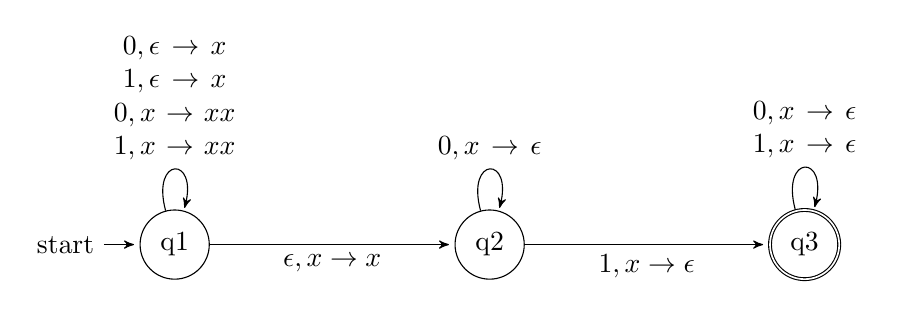
\begin{tikzpicture}[>=stealth',shorten >=2pt, auto, node distance=4cm]
	% Nodes {q1, q2, q3, q4, q5}
	\node [initial, state] 							(q1) 				{q1};
	\node [state] 									(q2) [right of=q1]  {q2};
	\node [state, accepting]  						(q3) [right of=q2]  {q3};

	% Paths
	\path [->]
	% Loop above paths
	(q1) edge [loop above] node	[text width=2cm, align=center]
	{$0, \epsilon \rightarrow x$ \\ $1, \epsilon \rightarrow x$ \\
	 $0, x \rightarrow xx$ \\ $1, x \rightarrow xx$}	(q1)
	(q2) edge [loop above] node	[text width=2cm, align=center]
	{$0, x \rightarrow \epsilon$}	(q2)
	(q3) edge [loop above] node	[text width=2cm, align=center]
	{$0, x \rightarrow \epsilon$ \\ $1, x \rightarrow \epsilon$}	(q3)

	% The paths between q1 and q2, as well as between q2 and q3
	(q1) edge [below]  node {$\epsilon, x \rightarrow x$} (q2)
	(q2) edge [below]  node {$1, x \rightarrow \epsilon$} (q3);

\end{tikzpicture} \\
\end{center}

\textbf{b.} Give a \textbf{CFG} that generates B. \\

We can give the \textbf{CFG} as follows:
$S \rightarrow UV$ \\
$U \rightarrow AB$ \\
$V \rightarrow A1A \; | \; A1B \; | \; A1U \; | \; B1U \; | \; U1U$ \\
$A \rightarrow 00^* \; | \; \in$ \\
$B \rightarrow 11^* \; | \; \in$ \\

This is because: \\
\textbf{1.} The string $s$ is a concatenation of $U$ and $V$. \\
\textbf{2.} The string $U$ can consist of any number of $0's$ and $1's$. \\
\textbf{3.} The string $V$ can consist of at least one $1$ or only $1$.\\
\textbf{4.} The string $A$ can consist of at least one $0$ or more than one $0's$. \\
\textbf{5.} The string $B$ can consist of at least one $1$ or more than one $1's$. \\

\end{document}
